\chapter{Задание 3. Гладим биржевые данные}
\label{ch:chap3}

\definecolor{codegreen}{rgb}{0,0.6,0}
\definecolor{codegray}{rgb}{0.5,0.5,0.5}
\definecolor{codepurple}{rgb}{0.58,0,0.82}
\definecolor{backcolour}{rgb}{0.95,0.95,0.92}

\lstdefinestyle{mystyle}{
    backgroundcolor=\color{backcolour},   
    commentstyle=\color{codegreen},
    keywordstyle=\color{magenta},
    numberstyle=\tiny\color{codegray},
    stringstyle=\color{codepurple},
    basicstyle=\ttfamily\footnotesize,
    breakatwhitespace=false,         
    breaklines=true,                 
    captionpos=b,                    
    keepspaces=true,                 
    numbers=left,                    
    numbersep=5pt,                  
    showspaces=false,                
    showstringspaces=false,
    showtabs=false,                  
    tabsize=2
}

\lstset{style=mystyle}

Выбираем какую-нибудь котировку ценной бумаги, у меня матлаб ругался на акции РосНефти по неизвестной мне причине, поэтому пришлось брать базовую базу, а именно всеми любимые зелёные бумажки (Сбербанк).
На этом \href{https://drive.google.com/drive/folders/1o8ozGv-bwYWuNpUlfYqM3rDu85QSQ0JW}{сайте} задали временной промежуток в 4 года и скачали \texttt{.csv} файл, с которым будем работать далее.

\section{Сравнительные графики исходного и фильтрованного сигналов}

\begin{figure}[ht]
    \centering
    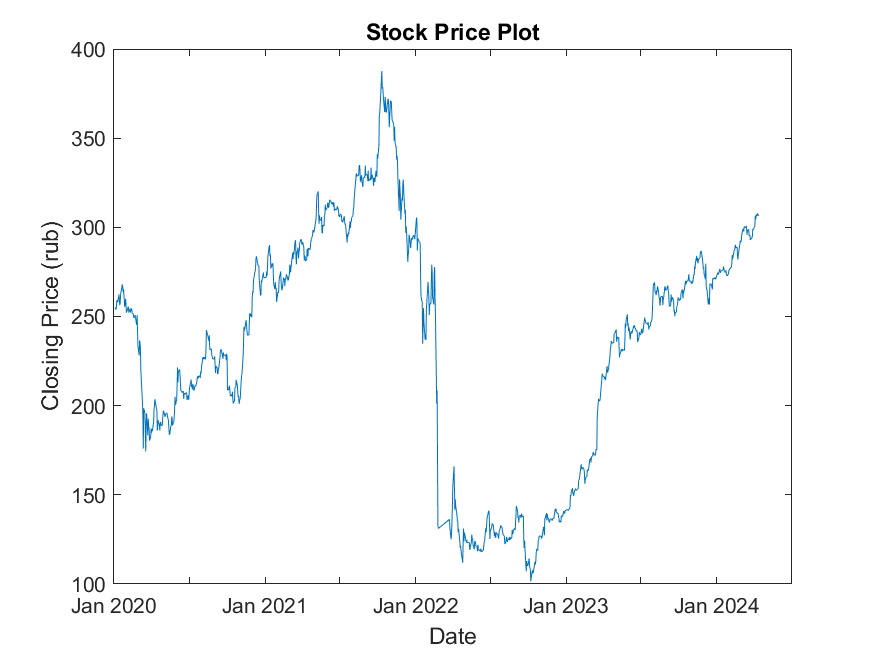
\includegraphics[width=0.8\textwidth]{test_stocks_original_SBER.png}
    \caption{Изначальный график котировки}
\end{figure}

\begin{figure}[ht]
    \centering
    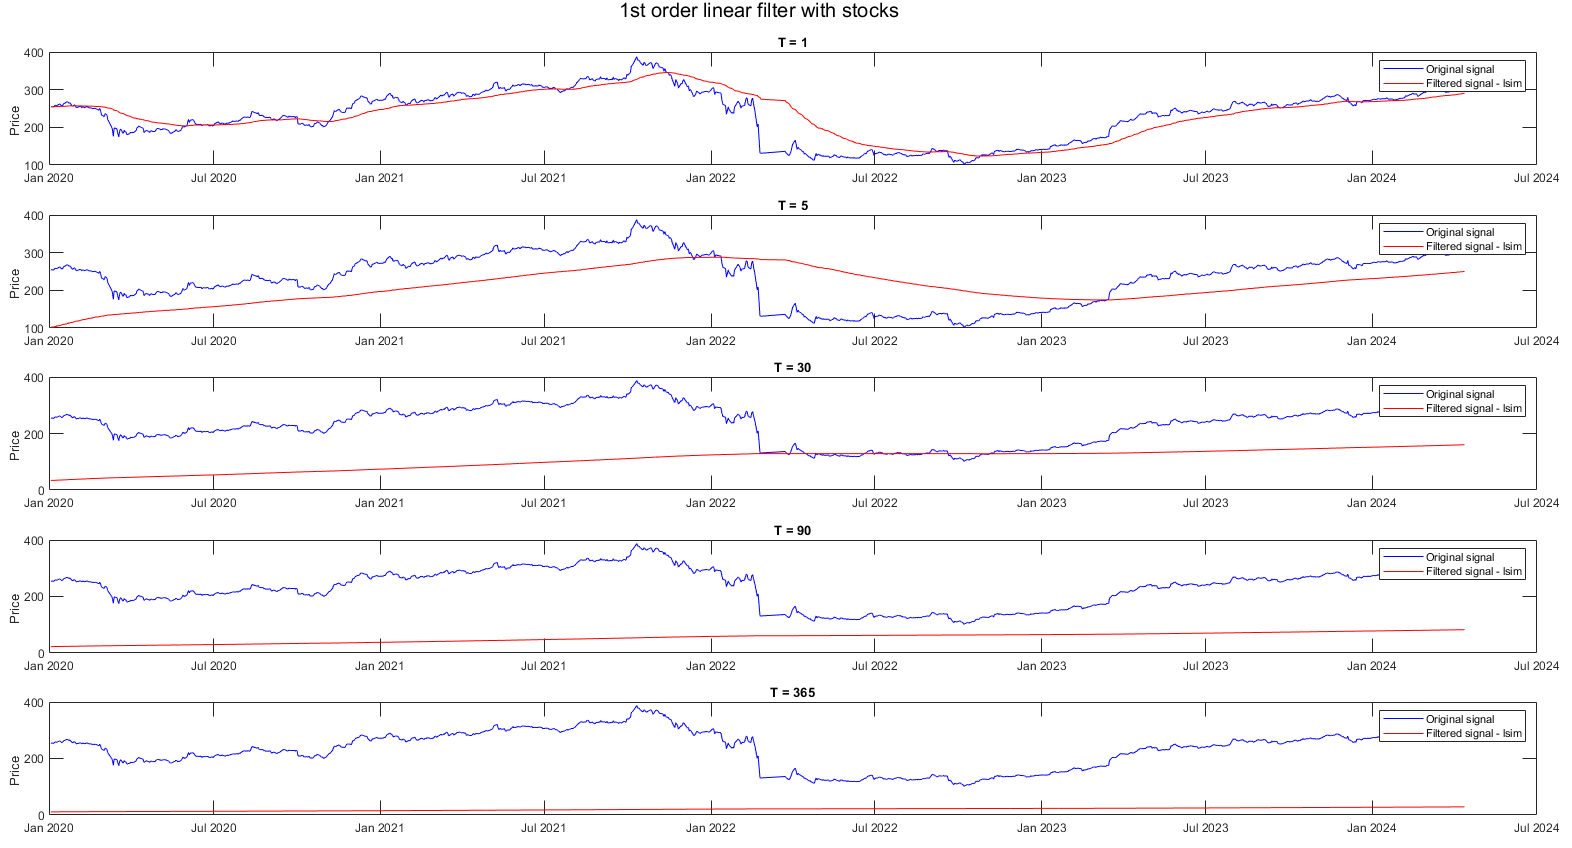
\includegraphics[width=1\textwidth]{untitled.png}
    \caption{Сглаживания по всем T}
\end{figure}


Получается, что каждый из подграфиков ниже нужно читать следующим образом: сначала мы сглаживаем "днями", то есть минимальный единичный отрезок при фильтрации на оси икс - это день, потом неделя, месяц, год. 
Так как данные у меня взяты за 4 года, то при апроксимации по годам итоговый график совсем плывёт и почти ничего не показывает, потому что для него слишком мало данных - всего 4 точки(4 года).

\endinput